\chapter{Множественная проверка гипотез}
\label{ch:multiple}

В главах~\ref{ch:basics}--\ref{ch:hypothesis} рассматривалась проверка одной гипотезы на уровне значимости $\alpha$.
Если выполнить $m$ независимых тестов при истинных $H_0$, вероятность хотя бы одной ошибки I рода растёт. При $\alpha=0{,}05$ и $m=20$ она уже превышает $0{,}64$.
Эта простая арифметика объясняет, почему значимые находки в массовых скринингах требуют отдельной интерпретации. Каждый отдельный тест контролирует вероятность ошибки I рода по одной гипотезе, тогда как исследователь зачастую интересуется семейством решений в целом.


На протяжении главы полезно возвращаться к трём вопросам из предисловия: постановка и допущения; применимость процедуры и графики; размер эффекта и альтернативные объяснения. 
Типичные ситуации множественной проверки --- сравнение нескольких алгоритмов классификации, скрининг дифференциальной экспрессии генов, поиск значимых корреляций в матрице признаков.
Настоящая глава вводит меры групповой ошибки~--- множественную ошибку первого рода (FWER) и ложную долю открытий (FDR)~--- и процедуры, которые контролируют эти величины.
Связь с главой~\ref{ch:hypothesis} прямая. Там изучались p-value и уровень значимости для одного теста. Здесь мы спрашиваем, что происходит, когда таких тестов десятки, тысячи или миллионы.
В главах~\ref{ch:anova} и~\ref{ch:regression} множественность снова возникнет при попарных сравнениях групп и при отборе предикторов. Процедуры настоящей главы задают общий язык для этих задач.

\section{Мотивирующие примеры}

Поиск экстрасенсов. В классическом эксперименте Джозефа Райна (Rhine, 1950) испытуемому предлагалось угадать цвет десяти карт, лежащих рубашкой вверх.
При $H_0$ (угадание наугад) число верных ответов $t$ имеет биномиальное распределение $Bi(10, 0{,}5)$.
Вероятность угадать $9$ или $10$ карт равна
\[ P(t\geq 9\mid H_0)=11\cdot 2^{-10}\approx 0{,}011.
\]
При одном испытании p-value $\approx 0{,}01$~--- основание для осторожного отклонения $H_0$, но не для сенсации.
Именно здесь важно различать уровень значимости одного теста и семейную ошибку. Если мы проводим тысячи экспериментов, редкое событие при $H_0$ становится почти неизбежным.

Из $1000$ испытуемых девять угадали $9$ карт и двое~--- все $10$. Ни один не подтвердил способности в повторных экспериментах.
Если экстрасенсов нет, вероятность найти хотя бы одного гениального случайно равна
\[ 1-\bigl(1-11\cdot 2^{-10}\bigr)^{1000}\approx 0{,}99998.
\]
Уже при $N=100$ эта вероятность превышает $1/2$.
Один значимый результат среди многих проверок~--- не доказательство эффекта, а типичное проявление множественной проверки.
Повторяемость, о которой шла речь в главе~\ref{ch:basics}, здесь критична. Без независимого подтверждения единичная значимость в массовом скрининге мало что доказывает.

Нейровизуализация и мёртвый лосось. В функциональной МРТ и ПЭТ-исследованиях гипотеза о различии активности мозга проверяется в каждом вокселе изображения. Их могут быть сотни тысяч или миллионы.
Без поправки на множественность значимые области возникают повсеместно, в том числе там, где биологически активности быть не может. Масштаб $m$ здесь принципиален. Даже при очень малом $\alpha$ произведение (много тестов) $\times$ (умеренный $\alpha$) даёт высокую семейную ошибку.

Команда Bennett и соавт. \citep{bennett2009} воспроизвела типичный fMRI-дизайн, где испытуемым служил мёртвый лосось. Ему показывали картинки с людьми в социальных ситуациях, затем сравнивали активность мозга с состоянием покоя.
Стандартный voxel-wise анализ без поправки выявил области, реагирующие на стимул.
Этот пример стал символом необходимости коррекции при массовом тестировании. Современные пакеты (SPM и аналоги) используют теорию гауссовых случайных полей и поправки на FWER/FDR.
Содержательный урок таков. Статистическая значимость в одном вокселе не эквивалентна научной значимости карты в целом. Без контроля семейной ошибки или FDR мы рискуем обнаружить активность там, где её быть не может.

С ростом $m$ растёт вероятность хотя бы одной ложной находки без поправки.
В нейровизуализации, геномике и скрининге алгоритмов множественная проверка~--- не опция, а обязательный этап интерпретации.
Типичный сценарий. Исследователь проводит $m=1000$ t-тестов, получает 47 значимых при $\alpha=0{,}05$ и хочет опубликовать список кандидатов. Без поправки ожидается $\approx 50$ ложных при полной $H_0$. BH с $\alpha=0{,}05$ сокращает список до устойчивых сигналов, а FWER-процедура (Холм) оставит лишь самые сильные находки.
Выбор между FDR и FWER~--- не технический, а этический. Допустима ли одна ложная регистрация лекарства среди десяти истинных?

\section{Проблема множественных сравнений}

Пусть имеются $m$ выборок (или $m$ подзадач), каждая со своей гипотезой.
Для гипотезы $H_i$ вычислена статистика $T_i$ и достигаемый уровень значимости $p_i$.
Важно. Величины $p_i$ сами по себе~--- случайные. При истинных $H_0$ они стремятся к равномерному распределению на $[0,1]$, а при ложных гипотезах смещаются к нулю. Множественная процедура~--- правило, которое по вектору $(p_1,\ldots,p_m)$ решает, какие индексы войдут в $\mathbf{R}$.
Обозначения.
\begin{itemize}
    \item $\mathbf{M}=\{1,\ldots,m\}$~--- множество всех индексов;
    \item $\mathbf{M}_0=\{i\colon H_i\ \text{верна}\}$, $|\mathbf{M}_0|=m_0$
(неизвестно исследователю);
    \item $\mathbf{R}=\{i\colon H_i\ \text{отвергнута}\}$, $|\mathbf{R}|=R$~---
множество отклонённых гипотез (управляемая величина);
    \item $V=|\mathbf{M}_0\cap\mathbf{R}|$~--- число ошибок I рода
          (ложных отклонений).
\end{itemize}

По аналогии с таблицей $2\times 2$ для одной гипотезы (глава~\ref{ch:basics}) составляют сводную таблицу (табл.~\ref{tab:mht-setup}).
Из всех её элементов исследователь знает только $m$. Остальные~--- случайные величины, зависящие от данных и выбранной процедуры.
Единственный рычаг~--- решить, какие гипотезы отвергать, то есть управлять $R$, стремясь удержать $V$ малым.
В отличие от одного теста, здесь нельзя одновременно наблюдать $V$ и $S$. Мы лишь выбираем пороги и правила отклонения, а истинное число ложных находок остаётся скрытым.

\begin{table}[htbp]
    \centering
    \caption{Сводная таблица множественной проверки гипотез}
    \label{tab:mht-setup}
    \footnotesize
    \begin{tabularx}{\linewidth}{|>{\raggedright\arraybackslash}X|>{\centering\arraybackslash}X|>{\centering\arraybackslash}X|>{\centering\arraybackslash}X|}
        \hline
        & Число верных $H_i$ & Число неверных $H_i$ & Всего \\
        \hline
        Число принятых $H_i$ & $U$ & $T$ & $m-R$ \\
        \hline
        Число отвергнутых $H_i$ & $V$ & $S$ & $R$ \\
        \hline
        Всего & $m_0$ & $m-m_0$ & $m$ \\
        \hline
    \end{tabularx}
\end{table}

Здесь $U$~--- верно принятые нулевые гипотезы, $T$~--- ошибки II рода (принятые ложные $H_0$), $S$~--- верно отвергнутые альтернативы.
Цель процедуры~--- дать гарантии на $V$ или на функцию от $V$ и $R$.
Выбор между FWER и FDR~--- это выбор между жёстким запретом хотя бы одной ложной находки и умеренным допуском нескольких ложных отклонений при контроле их доли среди всех отклонений.

\begin{definition}
Пусть проверяются гипотезы $H_1,\ldots,H_m$. Величина $V$~--- число ложных отклонений (отвергнутых истинных $H_0$), $R$~--- общее число отклонений.
Семейная ошибка первого рода (FWER) определяется как
\[ \FWER = \prob(V>0).
\]
\end{definition}

\begin{definition}
Ложная доля открытий (FDR) определяется как
\[ \FDR = \mathbb E\!\left[\frac{V}{\max(R,1)}\right].
\]
\end{definition}

FWER контролирует вероятность хотя бы одной ложной находки. FDR~--- ожидаемую долю ложных среди всех отклонённых гипотез.
Для любой процедуры $\FDR\leq\FWER$, поэтому контроль FDR менее консервативен и пропускает больше истинных эффектов.
Интуитивно. Если мы готовы терпеть, скажем, $5\%$ ложных среди списка кандидатов-генов, FDR-процедура уместна. Если же одна ложная регистрация лекарства недопустима, нужен контроль FWER.

\begin{remark}
При $m$ тестах без поправки ожидаемое число ложных отклонений составляет примерно $m_0\alpha$, где $m_0$~--- число истинных $H_0$.
На рис.~\ref{fig:bh-qq} видно типичное поведение p-value. Хвост малых значений смешивает истинные и ложные эффекты.
Без поправки мы не можем отделить случайный хвост от настоящих сигналов.
\end{remark}

\section{Контроль FWER}

Поправка Бонферрони. Одношаговая поправка Бонферрони отвергает $H_i$, если $p_i\leq \alpha/m$.

Эквивалентно. Сравнивают $p_i$ с $\alpha$ после замены $\tilde p_i=\min(1,\,m p_i)$.
Идея проста. Если все $H_i$ истинны, то при корректных $p_i$ вероятность ошибки по одной гипотезе не превышает $\alpha/m$, и неравенство Буля даёт $\FWER\leq\alpha$.
Практический смысл~--- разделить уровень значимости между $m$ тестами поровну, жертвуя мощностью ради жёсткого контроля ошибки.

Теорема. При любом совместном распределении $(p_1,\ldots,p_m)$ под истинными $H_0$ процедура обеспечивает $\FWER\leq\alpha$.
\begin{remark}[Эскиз доказательства]
Пусть $A_i=\{p_i\leq\alpha/m\}$ для $i\in\mathbf{M}_0$.
Тогда
\[ \FWER=\prob(V>0)=\prob\!\Bigl(\bigcup_{i\in\mathbf{M}_0} A_i\Bigr) \leq\sum_{i\in\mathbf{M}_0}\prob(A_i)\leq\sum_{i\in\mathbf{M}_0}\frac{\alpha}{m} =\frac{m_0}{m}\,\alpha\leq\alpha.
\]
Неравенство Буля завышает вероятность объединения событий, поэтому фактическая $\FWER$ часто существенно меньше $\alpha$. Процедура перестраховывается в отношении ошибки I рода и теряет мощность.
\end{remark}

Недостаток~--- консервативность. При росте $m$ мощность резко падает. Для двухвыборочного $t$-критерия ($\mu_1-\mu_2=1$, $\sigma=1$, целевая мощность $0{,}9$) требуемый объём выборки $n$ растёт с $m$.

\begin{table}[htbp]
    \centering
    \caption{Мощность при поправке Бонферрони ($\alpha=0{,}05$)}
    \label{tab:bonf-power}
    \begin{tabular}{|c|c|c|}
        \hline
        $m$ & $n$ & Мощность \\
        \hline
        $1$   & $23$  & $0{,}90$ \\
        $10$  & $23$  & $0{,}67$ \\
        $100$ & $23$  & $0{,}37$ \\
        $1000$& $23$  & $0{,}16$ \\
        $1000$& $62$  & $0{,}90$ \\
        \hline
    \end{tabular}
\end{table}

При $m=10^6$ и $n=10$ мощность $0{,}9$ достигается лишь при разнице средних порядка $5\sigma$.
Таблица~\ref{tab:bonf-power} наглядно показывает цену честности. При фиксированном $n$ рост $m$ превращает мощные одноразовые тесты в почти бесполезные. Восстановить мощность можно лишь увеличением объёма данных или переходом к менее консервативным процедурам.

Метод Холма. Метод Холма \citep{holm1979}~--- пошаговая нисходящая процедура.
Упорядочим $p_{(1)}\leq\cdots\leq p_{(m)}$ и отвергаем $H_{(i)}$ последовательно, пока $p_{(i)}\leq \alpha/(m-i+1)$.

Уровни значимости равны $\alpha_i=\alpha/(m-i+1)$, $i=1,\ldots,m$.

Модифицированные p-value задаются формулой
\[ \tilde p_{(i)}=\min\!\left(1,\;\max\!\bigl((m-i+1)p_{(i)},\,\tilde p_{(i-1)}\bigr)\right).
\]
Процедура контролирует $\FWER\leq\alpha$ без предположения о независимости $p_i$.
Метод Холма равномерно мощнее Бонферрони. При тех же данных он отвергает не меньше гипотез, поскольку $\alpha_i\geq\alpha/m$ для всех $i$.
Порядок имеет значение. Начиная с наименьших $p$, мы тратим часть бюджета $\alpha$ на самые убедительные отклонения, не применяя единый жёсткий порог $\alpha/m$ ко всем гипотезам сразу.
На практике скорректированные p-value Холма удобны для публикации. Гипотеза отвергается на уровне $\alpha$, если $\tilde p_i\leq\alpha$, при этом гарантия FWER сохраняется независимо от того, сколько гипотез исследователь просмотрел постфактум.
Для наглядности упорядочьте четыре p-value $(0{,}001,\ 0{,}03,\ 0{,}04,\ 0{,}08)$ при $m=4$, $\alpha=0{,}05$. Холм отвергает первые три гипотезы (пороги $0{,}0125$, $0{,}0167$, $0{,}025$), четвёртая остаётся. Бонферрони потребовал бы $p\leq 0{,}0125$ для каждой~--- отвергли бы только первую. Разница в мощности заметна на малом $m$ и усиливается при росте числа тестов.

Нисходящие и восходящие процедуры. Обобщённая схема stepwise-процедур использует вариационный ряд $p_{(1)}\leq\cdots\leq p_{(m)}$ и индивидуальные пороги $\alpha_i$.

Нисходящая процедура (Холм, Бонферрони) начиная с $p_{(1)}$ отвергает $H_{(i)}$, пока $p_{(i)}\leq\alpha_i$. При первом нарушении принимаются все оставшиеся гипотезы.

Восходящая процедура (BH, BY) начиная с $p_{(m)}$ принимает $H_{(i)}$, пока $p_{(i)}>\alpha_i$. При первом нарушении отвергаются $H_{(1)},\ldots,H_{(i)}$.

При одних и тех же $\alpha_i$ восходящая процедура отвергает не меньше гипотез, чем нисходящая.
FWER-процедуры~--- преимущественно нисходящие. FDR-процедуры~--- восходящие.
Уровни Холма ($\alpha_i=\alpha/(m-i+1)$) убывают по гиперболе. Уровни BH ($\alpha_i=\alpha i/m$) растут линейно от $\alpha/m$ до $\alpha$.
Эта асимметрия отражает различие целей. FWER останавливается при первой сомнительной гипотезе. FDR набирает отклонения от малых $p$ к большим, пока маленькие p-value оправдывают расширение списка открытий.
Stepwise-процедуры можно представить как последовательное применение правила отвергнуть или принять к упорядоченным p-value. Различие лишь в направлении обхода и в том, что происходит после первого нарушения порога.
При первом знакомстве с BH часто возникает вопрос, почему порог растёт с $i$. Ответ содержательный. Мы разрешаем больше отклонений среди гипотез с малыми $p$, но контролируем долю ложных среди всего списка отклонений, а не вероятность хотя бы одной ошибки. FWER-логика обратна. Первое сомнительное $p$ останавливает цепочку отвержений.

Модельный эксперимент. Сгенерированы $m=200$ выборок объёма $n=20$. $150$ из $N(0,1)$ (истинные $H_0$) и $50$ из $N(1,1)$ (истинные альтернативы).
Для каждой проверяется $H_i\colon\mathbb EX_i=0$ одновыборочным $t$-критерием (табл.~\ref{tab:model-mht}).
Эксперимент имитирует скрининг, где лишь четверть гипотез истинно альтернативна~--- типичная для геномики пропорция.

\begin{table}[htbp]
    \centering
    \caption{Результаты модельного эксперимента ($m=200$, $m_0=150$)}
    \label{tab:model-mht}
    \footnotesize
    \begin{tabularx}{\linewidth}{|>{\raggedright\arraybackslash}X|>{\centering\arraybackslash}X|>{\centering\arraybackslash}X|>{\centering\arraybackslash}X|}
        \hline
        & Верных $H_i$ & Неверных $H_i$ & Всего \\
        \hline
        \multicolumn{4}{|l|}{\textsc{Без поправки}} \\
        \hline
        Принято & $142$ & $0$ & $142$ \\
        Отвергнуто & $8$ & $50$ & $58$ \\
        \hline
        \multicolumn{4}{|l|}{\textsc{Бонферрони}} \\
        \hline
        Принято & $150$ & $27$ & $177$ \\
        Отвергнуто & $0$ & $23$ & $23$ \\
        \hline
        \multicolumn{4}{|l|}{\textsc{Холм}} \\
        \hline
        Принято & $150$ & $24$ & $174$ \\
        Отвергнуто & $0$ & $26$ & $26$ \\
        \hline
        \multicolumn{4}{|l|}{\textsc{BH ($\alpha=0{,}05$)}} \\
        \hline
        Принято & $148$ & $4$ & $152$ \\
        Отвергнуто & $2$ & $46$ & $48$ \\
        \hline
        \multicolumn{4}{|l|}{\textsc{BY ($\alpha=0{,}05$)}} \\
        \hline
        Принято & $150$ & $10$ & $160$ \\
        Отвергнуто & $0$ & $40$ & $40$ \\
        \hline
    \end{tabularx}
\end{table}

Без поправки восемь ложных отклонений среди $150$ истинных $H_0$ согласуются с ожиданием $m_0\alpha\approx 7{,}5$.
Бонферрони и Холм не допускают ни одной ошибки I рода, но пропускают часть истинных эффектов. BH находит компромисс, допуская две ложные находки при существенно большем числе верных отклонений.
Сравнение BY с BH в этом эксперименте показывает типичный компромисс. BY консервативнее (40 против 48 отклонений), но при зависимых тестах даёт более надёжную верхнюю границу FDR.
Эксперимент воспроизводят по той же схеме: матрица $200\times 20$, $t$-тест по каждому столбцу, затем поправки Бонферрони, Холма, BH и BY --- в любом статистическом пакете курса.

FWER-процедуры уместны, когда цена единственной ложной находки высока. Регистрация лекарства, юридические выводы, подтверждение единственной научной гипотезы среди многих второстепенных.
При чистом исследовательском скрининге (гены, SNP) допустима более мягкая FDR-процедура.

\section{Контроль FDR}

Процедура Бенджамини--Хохберга. Процедура BH \citep{benjamini1995} (Бенджамини--Хохберга, восходящая) находит наибольший $k$, для которого $p_{(k)}\leq \frac{k}{m}\alpha$, и отвергает $H_{(1)},\ldots,H_{(k)}$.

Эквивалентная формулировка через модифицированные p-value:
\[ \tilde p_{(i)}=\min\!\left(1,\;\min_{j\geq i}\frac{m}{j}\,p_{(j)}\right).
\]
При независимых (или с положительной регрессионной зависимостью) $p_i$ процедура обеспечивает $\FDR\leq\alpha$.
В отличие от Холма, BH не контролирует FWER безусловно. Она допускает несколько ложных отклонений, но ограничивает их ожидаемую долю среди всех отклонённых.
Условие контроля FDR~--- независимость $p_i$ или свойство положительной регрессионной зависимости (ПРЗ) на подмножестве истинных $H_0$. Для многомерного нормального распределения с неотрицательными корреляциями ПРЗ выполняется.
Практически BH часто применяют в геномике именно потому, что исследователь готов интерпретировать список кандидатов, зная, что лишь небольшая доля из них может оказаться ложной.
Пороговая линия $p_{(i)}=i\alpha/m$ на QQ-plot p-value наглядно показывает, сколько гипотез BH отвергает. Все точки под этой линией попадают в список отклонений.

Процедура Бенджамини--Йекутиели. Процедура BY \citep{benjamini2001}~--- восходящая процедура с уровнями
\[ \alpha_i=\frac{\alpha\, i}{m\sum_{j=1}^{m}1/j},\qquad \tilde p_{(i)}=\min\!\left(1,\;\min_{j\geq i}\frac{m\sum_{k=1}^{m}1/k}{j}\,p_{(j)}\right).
\]
Контролирует $\FDR\leq (m_0/m)\alpha\leq\alpha$ при любой зависимости между $p_i$. При отсутствии информации о зависимости метод неулучшаем среди FDR-процедур.
При малой доле ложных гипотез BY консервативнее BH и может отвергать меньше находок, чем даже FWER-процедура Холма.
Когда тесты сильно зависимы (соседние гены, коррелированные воксели), BY даёт теоретически обоснованную страховку там, где BH может завышать FDR.
Коэффициент $\sum_{j=1}^{m}1/j\approx \ln m + \gamma$ делает пороги BY существенно строже, чем у BH, при больших $m$. Это плата за универсальность гарантии при произвольной зависимости.

$q$-значения и оценка $m_0$. Процедура Storey оценивает долю истинных $H_0$ по хвосту распределения p-value:
\[ \hat\pi_0(\lambda)=\frac{1+\#\{i\colon p_i>\lambda\}}{(1-\lambda)m}, \qquad \hat m_0=m\,\hat\pi_0(\lambda),
\]
где $\lambda\in[0,1)$~--- порог (часто $\lambda=0{,}5$).
$q$-значение гипотезы $H_i$~--- минимальный уровень FDR, при котором $H_i$ ещё можно отвергнуть. Это FDR-аналог скорректированных p-value.
Оценка $\hat m_0$ имеет положительное смещение и большую дисперсию при коррелированных $p_i$, поэтому для контроля FWER напрямую не применяется. $q$-значения удобны при интерпретации списка кандидатов в геномике.
Интерпретация $q=0{,}05$ для гена такова. Если включить этот ген в список отклонённых при целевом FDR $5\%$, ожидаемая доля ложных среди всех отклонённых на этом уровне не превышает $5\%$. Это отличается от утверждения, что $p=0{,}05$ означает 5\% риска для этой гипотезы.
Пример с мутацией и фамилией показывает, что множественность~--- это не только много генов, но и любое семейство гипотез, сформулированных до просмотра данных. Включение заведомо лишней проверки в то же семейство ужесточает порог для содержательной гипотезы~--- аргумент за предварительную регистрацию протокола и за разделение подтверждающего и разведочного анализов.

Следующие ошибки интерпретации встречаются особенно часто при переходе от одиночных тестов (глава~\ref{ch:hypothesis}) к массовому скринингу.
\begin{itemize}
    \item Проводить $m$ тестов и отвергать все с $p_i<0{,}05$ без поправки,
          затем интерпретировать каждое отклонение как значимое открытие.
    \item Применять BH при сильной положительной корреляции статистик
          без проверки условий. FDR может быть завышен.
    \item Считать, что контроль FDR на уровне $0{,}05$ означает
          вероятность ошибки 5\% для каждой отвергнутой гипотезы. FDR~--- ожидание доли, а не маргинальная вероятность.
\end{itemize}

Ложные гипотезы маскируют истинные эффекты. Рассмотрим исследование связи болезни с мутацией и с фамилией на гласную (табл.~\ref{tab:mutation}).
Мутация встречается у $1$ из $100$ здоровых и $8$ из $100$ больных ($p\approx 0{,}035$). Фамилия на гласную~--- $p\approx 0{,}66$.

\begin{table}[htbp]
    \centering
    \caption{Две гипотезы в одном исследовании}
    \label{tab:mutation}
    \footnotesize
    \begin{tabularx}{\linewidth}{|>{\raggedright\arraybackslash}X|c|c|c|}
        \hline
        & Контроль ($100$) & Больные ($100$) & $p$ \\
        \hline
        Мутация & $1$ & $8$ & $0{,}035$ \\
        Фамилия на гласную & $36$ & $40$ & $0{,}66$ \\
        \hline
    \end{tabularx}
\end{table}

При $m=2$ любая FWER/FDR-процедура сравнивает наименьший p-value с $\alpha/2=0{,}025$. Мутация не проходит порог. Нелепая вторая гипотеза повышает цену первой~--- ещё один аргумент за предварительный отбор гипотез до сбора данных.
Содержательно. Включение заведомо бессмысленных проверок в одно семейство ухудшает шансы содержательных гипотез, даже если по ним есть реальный сигнал.

Анализ подгрупп. При сравнении выживаемости по $6$ подгруппам факторов (Lee et al., 1980) в одной подгруппе обнаружено значимое преимущество лечения~B, хотя оба лечения были идентичны (различались лишь названия).
При $\approx 50$ подгруппах (Ishitani, Lin, 2008, кофеин и рак груди) легко получить несколько открытий с $p$ около $0{,}02$--$0{,}08$ без поправки~--- аналог переобучения на подвыборках.
Здесь пересекаются две линии рассуждений из главы~\ref{ch:multiple}. Формальная поправка на $m$ подгрупп и содержательное ограничение числа подгрупп, заданных до просмотра данных.
Апостериорно найденные подгруппы почти неизбежно выглядят значимыми даже при отсутствии эффекта в генеральной совокупности.

Лучшая защита от множественности~--- проверять меньше гипотез, заранее отфильтровав содержательно неинтересные. Фильтрация после просмотра p-value недопустима.
При зависимых тестах (соседние гены, коррелированные признаки) используют BY или подходы на основе перестановок. При известном совместном нулевом распределении~--- параметрические процедуры (HSD Тьюки, критерий Даннета), которые мы встретим в главе~\ref{ch:anova}.
Множественность~--- свойство постановки, а не техническая поправка в конце. Если исследователь заранее ограничит число гипотез и разделит подтверждающий и разведочный анализ, формальная процедура работает в более благоприятном режиме, чем при тысяче тестов, сформулированных апостериорно.

\section{Примеры}
\label{sec:examples}

Сравнение классификаторов. В таблице AUC классификаторов приведены AUC четырёх вариантов дерева решений C4.5 на $m=14$ наборах данных.
Для каждого набора можно проверить $H_0\colon \text{AUC}_A=\text{AUC}_B$ (например, базовый C4.5 против C4.5+m).

При $m=14$ поправка Бонферрони требует $p\leq 0{,}05/14\approx 0{,}0036$.
Метод Холма последовательно ослабляет порог. BH допускает больше отклонений при контроле FDR.
Содержательный вывод. Улучшения на отдельных наборах (mushroom, iris) не обязаны обобщаться~--- множественная проверка защищает от cherry-picking лучших строк таблицы.
Задача типична для сравнительных исследований в главе~\ref{ch:basics}. Мы повторяем один и тот же статистический тест на множестве датасетов и должны отделить устойчивое преимущество от случайных всплесков AUC.
Содержательная интерпретация требует не только значимости на iris, но и вопроса. Если алгоритм лучше на $3$ из $14$ наборов после поправки, достаточно ли этого для рекомендации в продакшене?
Множественная проверка отвечает на статистическую часть вопроса. Принятие решения остаётся за экспертом по предметной области.
При сравнении классификаторов полезно явно разделить два уровня. (1)~Алгоритм A лучше B на наборе iris после поправки?~--- статистический вопрос с FWER/FDR. (2)~Стоит ли внедрять A в промышленную эксплуатацию?~--- вопрос о стабильности на новых данных и стоимости, который поправка на множественность не решает. Такой двухуровневый разбор предотвращает подмену бизнес-решения списком скорректированных p-value.

Дифференциальная экспрессия генов. В наборе p-value дифференциальной экспрессии приведены p-value для $m=50$ генов.
Без поправки $17$ генов значимы при $\alpha=0{,}05$. Это ожидаемо даже при полном отсутствии эффектов ($50\times 0{,}05=2{,}5$ ложных в среднем).

\begin{figure}[htbp]
    \centering
    
\includegraphics[width=\FigWidth]{\FigDir/chapter-3/ps_adj_bh.png}
    \caption{QQ-plot наблюдаемых p-value против равномерного
    распределения. Отклонение от диагонали у малых $p$ указывает
    на наличие истинных эффектов.}
    \label{fig:bh-qq}
\end{figure}

Применение процедур.
\begin{itemize}
    \item Бонферрони ($p_i\leq 0{,}001$). Отвергаются $4$ гипотезы.
    \item Холм. Отвергаются $4$ гипотезы (не меньше Бонферрони).
    \item BH ($\alpha=0{,}05$). Отвергаются $8$ гипотез,
          включая гены с наименьшими p-value.
\end{itemize}

На рис.~\ref{fig:bh-qq} видно, что часть p-value существенно меньше ожидаемых при полной нулевой гипотезе~--- именно их BH идентифицирует как кандидатов на дифференциальную экспрессию, контролируя ожидаемую долю ложных среди отклонённых.
QQ-plot~--- полезный диагностический шаг перед выбором процедуры. Если весь хвост лежит на диагонали, возможно, истинных эффектов нет и любая поправка лишь сократит ложные находки. Если хвост резко отклоняется к малым $p$, сигнал есть и FDR-процедура поможет отделить его от шума.
В биоинформатике список из восьми генов после BH часто передаётся на функциональную аннотацию (GO, KEGG). $q$-значение каждого гена ранжирует приоритеты для дорогостоящей экспериментальной валидации.

Скрининг 500 SNP. Пусть в case--control исследовании для $m=500$ SNP получены p-value (независимость~--- идеализация. На практике SNP коррелированы, но схема иллюстративна). Без поправки 31 SNP имеют $p<0{,}05$. При $m_0\approx 480$ истинных $H_0$ ожидаем $\approx 24$ ложных~--- число 31 лишь слегка превышает шум, но исследователь может ошибочно принять весь список за находки.

Бонферрони ($\alpha/500=0{,}0001$) оставляет 4 SNP. Холм~--- 5. BH при FDR $=0{,}05$~--- 11. QQ-plot показывает, что хвост заметно отклоняется от диагонали~--- есть сигнал сверх шума, но не все 31 значимость устойчивы. $q$-значение ранжирует SNP для дальнейшей валидации на независимой выборке.

FWER-процедура защищает от ложной публикации единичного SNP. FDR формирует список кандидатов с контролируемой долей ложных. Выбор зависит от цены ошибки. Для клинического отчёта об одном SNP разумен Холм. Для омикс-скрининга~--- BH и воспроизведение. Глава~\ref{ch:hypothesis} ввела p-value. Настоящая глава показывает, что семейство таких p-value требует отдельной логики. Иначе множественность превращает 5\%-й уровень в иллюзию.

В публикации указывают число тестов $m$, целевую величину (FWER или FDR) и уровень $\alpha$, метод (Холма, BH, BY), число отклонений до и после поправки, QQ-plot или гистограмму p-value.
Скорректированное $p$ или $q$-значение прикладывают к полному списку гипотез, а не только к значимым~--- иначе читатель не может воспроизвести процедуру. При подтверждающем анализе семейство гипотез фиксируют до сбора данных. Разведочный блок~--- отдельно, с более мягким FDR и без утверждения о доказанности.

Попарные сравнения после ANOVA (гл.~\ref{ch:anova}, HSD Тьюки) и отбор предикторов в регрессии (гл.~\ref{ch:regression}, пошаговые $t$-тесты)~--- те же семейства гипотез, что геномного скрининга SNP или сравнение классификаторов. Различие лишь в масштабе $m$ и в цене ошибки. Тьюки контролирует FWER для запланированных контрастов. BH~--- FDR для скрининга. Умение выбрать процедуру по постановке исследования~--- главный практический итог главы.

При $m\le 10$ разница Холма и BH часто мала. При $m\ge 10^3$ Бонферрони может обнулить мощность, а BH~--- единственный практичный FDR-контроль.
При коррелированных тестах (SNP, воксели) BY или методы на основе перестановок предпочтительнее наивного BH. QQ-plot p-value помогает отличить наличие сигнала от чистого шума. Запишите $m$ и процедуру в заголовке таблицы результатов.

Один значимый SNP после BH на выборке открытия требует воспроизведения на независимой когорте. Иначе FDR контролирует лишь ожидаемую долю ложных в списке, а не гарантию для каждого SNP. В мета-анализе p-value объединяют по схемам Фишера/Стаффера с отдельной поправкой на число исследований. Типичная цепочка~--- открытие, поправка, воспроизведение, содержательный механизм.

\section{Дополнительные процедуры FWER и FDR}

Одношаговая поправка Шидака. При независимых (или positive lower orthant dependent) статистиках $t_i$ одношаговая процедура Шидака задаёт общий уровень
\[ \alpha_i = 1-(1-\alpha)^{1/m},\qquad i=1,\ldots,m,
\]
и отвергает $H_i$, если $p_i\leq\alpha_i$.
Эквивалентно сравнивают модифицированные достигаемые уровни
\[ \tilde p_i = 1-(1-p_i)^m.
\]
Идея. При истинных $H_0$ и независимых $p_i$ вероятность хотя бы одной ошибки I рода равна $1-(1-\alpha_i)^m=\alpha$.
При больших $m$ пороги Шидака чуть мягче, чем у Бонферрони ($\alpha/m$), поэтому процедура менее консервативна, но требует независимости.

Поправка Шидака (одношаговая): пороги $\alpha_i = 1-(1-\alpha)^{1/m}$, отвергают $H_i$ при $p_i\leq\alpha_i$; модифицированные $p_i = \min(1,1-(1-p_i)^m)$; при независимых $p_i$ $\FWER\leq\alpha$.

Нисходящая процедура Шидака--Холма. Шидак--Холм~--- пошаговая нисходящая аналог Холма с уровнями
\[ \alpha_i = 1-(1-\alpha)^{1/(m-i+1)},\qquad \tilde p_{(i)} = \max\!\left( 1-(1-p_{(i)})^{m-i+1},\; \tilde p_{(i-1)} \right).
\]
При независимых $p_i$ это наиболее мощная известная FWER-процедура. На практике при $m\gtrsim 20$ пороги близки к Холму (см. рис.~порогов $\alpha_i$ в лекции~4).

Шидак--Холм: пошаговая нисходящая процедура с $\alpha_i = 1-(1-\alpha)^{1/(m-i+1)}$; при независимых $p_i$ наиболее мощная известная FWER-процедура.

Перестановочная множественная проверка. Когда $p_i$ сильно зависимы (соседние воксели, коррелированные гены), универсальные поправки (Холм, BY) теряют мощность.
Перестановочные методы \citep{westfall2008} строят совместное нулевое распределение вектора $(T_1,\ldots,T_m)$ эмпирически.
\begin{enumerate}
    \item Зафиксировать наблюдаемые $T_i^{\text{obs}}$.
    \item $B$ раз сгенерировать перестановки данных, сохраняющие
          структуру $H_0$ (перестановка меток классов, столбцов таблицы и~т.\,п.).
    \item Для каждой перестановки $b$ вычислить $T_i^{(b)}$.
    \item Оценить скорректированные p-value. Доля перестановок, где
          $\max_i T_i^{(b)}\geq\max_i T_i^{\text{obs}}$ (или пошаговая нисходящая max-$T$ по схеме Westfall--Young).
\end{enumerate}
Требуется subset pivotality. Нулевое распределение подмножества статистик не зависит от истинности остальных $H_0$.
Примеры. Попарные сравнения нормальных групп, линейные контрасты средних, коррелированные нормальные выборки (Bretz, гл.~5).

Перестановочный max-$T$: эмпирическое нулевое распределение $M=\max_i T_i$ по $B$ перестановкам, сохраняющих $H_0$; требуется subset pivotality.

Cherry-picking и FDP. В отличие от BH, где контролируется $\FDR=\mathbb E[V/\max(R,1)]$, подход cherry-picking \citep{goeman2011} позволяет после просмотра данных выбрать произвольное множество отклонений $\mathbf{R}\subseteq\{1,\ldots,m\}$ и оценить верхнюю границу ложной доли среди выбранных:
\[ \FDP = \frac{V}{R},\qquad R=|\mathbf{R}|.
\]
Оценка справедлива одновременно для всех $2^m-1$ возможных $\mathbf{R}$, что удобно, когда в список кандидатов (мутации, гены) входят и объекты с малыми $p_i$, и объекты по экспертным соображениям.
Важно не путать. FDP~--- доля в конкретном выбранном списке. FDR~--- ожидание доли по процедуре.
Cherry-picking в сравнении классификаторов (гл.~\ref{ch:multiple}, \S\ref{sec:examples}) означает отчёт только о лучших строках таблицы AUC без поправки~--- формально это апостериорный выбор $\mathbf{R}$, не контролирующий ни FWER, ни FDR.

\begin{remark}
Процедуры Goeman и соавт. дают одновременные верхние границы FDP для семейства подмножеств. Детали~--- в обзоре \citet{goeman2014}.
\end{remark}

\section{Практика и семинар}
\label{sec:practice-ch3}


\PracticeIntro{4}
$m=200$, $m_0=150$ истинных $H_0$.
Напоминание: $\FWER=\prob(V>0)$~--- хотя бы одна ложная находка среди истинных $H_0$; FDR~--- ожидаемая доля ложных среди всех отклонений (см. начало главы и табл.~\ref{tab:model-mht}).

\paragraph{Без поправки.}
\textbf{Постановка.} $m=200$ столбцов, у 150 --- чистый шум $N(0,1)$.
\textbf{График.} Гистограмма $p$-value (рис.~\ref{fig:p3-pval}): хвост малых $p$ при отсутствии эффектов в большинстве столбцов.
\begin{figure}[htbp]
\centering
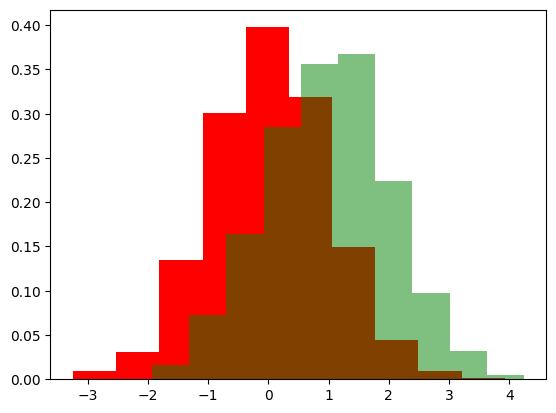
\includegraphics[width=\FigWidth]{figures/practice/chapter-3/sem4-cell10-out0.png}
\caption{Семинар~4: распределение $p$-value. На графике виден избыток малых $p$ слева.}
\label{fig:p3-pval}
\end{figure}
\textbf{Числа.} Без поправки отклоняют $\approx 50$ гипотез; ложных среди $H_0$ $\approx 7$--8 (ожидание $m_0\alpha\approx 7{,}5$).
\medskip\noindent\textbf{Три вопроса.} \textit{Постановка:} $m$ одновременных $t$-тестов. 
\textit{Применимость:} наивный порог $p<\alpha$ --- только иллюстрация; для отчёта нужна поправка. 
\textit{Вывод:} часть «значимостей» --- шум при множественности.\medskip

\paragraph{С поправкой.}
См. табл.~\ref{tab:model-mht} и пороги на рис.~\ref{fig:p3-thresh}: Holm/Bonferroni не допускают ложных среди $H_0$; BH --- компромисс FDR.
\begin{figure}[htbp]
\centering
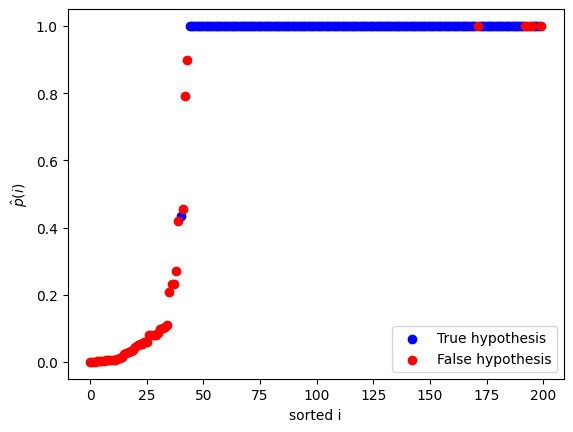
\includegraphics[width=\FigWidth]{figures/practice/chapter-3/sem4-cell27-out0.png}
\caption{Семинар~4: пороги Holm и BH. Обратите внимание, что BH отсекает больше малых $p$, чем строгий FWER.}
\label{fig:p3-thresh}
\end{figure}
\medskip\noindent\textbf{Три вопроса.} \textit{Постановка:} то же семейство из $m$ тестов. 
\textit{Применимость:} Holm при высокой цене ложной находки; BH при списке кандидатов. 
\textit{Вывод:} сообщить метод, число отклонений и смысл FDR.\medskip

\paragraph{Классификаторы (\S\ref{sec:examples}).}
Сравнение AUC на $m=14$ наборах: без поправки легко «найти» победу на iris; после Holm/BH устойчивых побед меньше --- тот же cherry-picking, что в таблице теории.
\medskip\noindent\textbf{Три вопроса.} \textit{Постановка:} $m$ парных сравнений алгоритмов. 
\textit{Применимость:} поправка на семейство до выбора «лучшего» датасета. 
\textit{Вывод:} одна строка таблицы AUC не лицензирует внедрение в прод.\medskip

По итогам: $m$, $\alpha$, метод, ложные без поправки, цена FWER, смысл BH.

\section{Контрольные вопросы по теме}

\begin{enumerate}
    \item При $m=100$ и $\alpha=0{,}05$ оцените вероятность хотя бы
          одной ошибки I рода без поправки, если все $H_i$ истинны и тесты независимы.
    \item Сформулируйте метод Холма для $m=4$ и порога $\alpha=0{,}05$
          с p-value $(0{,}001,\ 0{,}03,\ 0{,}04,\ 0{,}08)$.
          Сколько гипотез будет отвергнуто?
    \item Чем восходящая процедура BH принципиально отличается
          от нисходящей процедуры Холма?
    \item Почему $\FDR\leq\FWER$ для любой процедуры? Приведите
          содержательный пример, когда FDR-процедура предпочтительнее.
    \item Для дифференциальной экспрессии объясните, почему число
          отвержений BH ($8$) превышает число отклонений Холма ($4$).
    \item Сравните уровни значимости Холма и BH при $m=10$, $\alpha=0{,}05$.
          Сколько гипотез отвергнёт каждая процедура при p-value $(0{,}001,\ 0{,}02,\ 0{,}03,\ 0{,}04,\ 0{,}05,\ 0{,}06,\ 0{,}1,\ 0{,}2,\ 0{,}5,\ 0{,}8)$?
    \item Чем процедура BY отличается от BH? Когда BY предпочтительнее?
    \item Объясните, почему $q$-значение удобнее сырого p-value при
          скрининге $5000$ генов.
    \item Почему анализ $50$ подгрупп без поправки напоминает
          переобучение?
    \item Верно ли, что «p-value $=0{,}03$ означает, что $H_0$ верна с вероятностью 3\%»? Объясните.
    \item Сравните поправки Бонферрони и Шидака. При каких условиях Шидак менее консервативен?
    \item Чем FDP отличается от FDR? Почему cherry-picking без поправки не контролирует ни FWER, ни FDR?
\end{enumerate}
